%\documentclass[11pt,twoside,openany]{is2}
\documentclass[11pt,twoside,openright]{is2}
%%
%% TOGGLE TO MAKE REMARKS VISIBLE
%%
%%\newcommand{\remark}[1]{\begin{quotation}\textit{#1}\end{quotation}}
%%\newcommand{\remark}[1]{}

\usepackage[hyperfootnotes=false, colorlinks=false, pdfborder={0 0 0}]{hyperref}
\usepackage{psfrag}
\usepackage{graphics}
\usepackage{graphicx}
\graphicspath{{figures/}}    % location of images and graphics % added by me (Lovis)
\usepackage{amssymb}
%\usepackage[T1]{fontenc}
%\usepackage[latin1]{inputenc}
\usepackage[english]{babel}
\usepackage{enumitem}
\usepackage{boxedminipage}
\setlength{\fboxsep}{4mm}
\usepackage{float}
\usepackage{hyperref}
%\usepackage{float}
%\usepackage{afterpage}
%\usepackage{subfigure}
%\usepackage{theorem}
%\usepackage{tabularx}
%\usepackage{helvet}
%\usepackage{a4wide}
\usepackage{times}
%\usepackage{palatino}
\usepackage{makeidx}
\usepackage{amsmath}
\usepackage{amssymb}
%\usepackage{mathptm}
%\usepackage{moreverb}
%\usepackage{picinpar}
%\usepackage{fancyhdr}
%\usepackage{alltt}
%\usepackage{fancybox}
%\usepackage{eepic}
\usepackage{wrapfig}
\usepackage{epsfig}
%\usepackage{doxygen}
\usepackage{hangcaption}
%\usepackage[dvips]{rotating}
\usepackage{rotating}
\usepackage[hang]{subfigure}
\usepackage{algo}
%\usepackage{textcomp,xspace}
\usepackage{listings}

% Added by me (Lovis):
%\usepackage{natbib} % to use \citet
%\usepackage{mathtools}
%\usepackage{tikz}
%\usepackage{pgfplots}
%\pgfplotsset{compat=1.17}
%\usepackage{enumitem}
\usepackage{tabularx}
\newcolumntype{L}[1]{>{\raggedright\arraybackslash}X{#1}} % linksbündig ohne Breitenangabe in tabularx-X-style
\newcommand{\ctab}{\centering\arraybackslash} % Tabellenabschnitt zentriert in tabularx
\usepackage{threeparttable}
%\usepackage{multirow}
%\usepackage{showframe}
% End (Lovis)

%% Abbreviations added by me (Lovis)
\RequirePackage{xspace}
\newcommand{\ie}{i.e.\@\xspace}
\newcommand{\eg}{e.g.\@\xspace}
\newcommand{\Eg}{E.g.\@\xspace}
%\newcommand{\etc}{etc.\@\xspace}
\newcommand{\wrt}{w.r.t.\@\xspace}
\newcommand{\cf}{cf.\@\xspace}
\newcommand{\etal}{et~al.\@\xspace}
\newcommand{\iA}{i.a.\@\xspace}
% End (Lovis)

%\renewcommand{\sfdefault}{cmss}

\renewcommand{\floatpagefraction}{0.75}
\sloppy
\setlength{\parskip}{2pt} 
\setlength{\parindent}{0pt} 

%\pagestyle{headings}
%\makeindex

\setcounter{tocdepth}{2}
\hyphenation{ana-ly-sis opera-tion opera-tions opera-tio-nal neglected}


\newcommand{\rot}[1]{

\begin{rotate}{-60}

#1

\end{rotate}

}


\newcommand{\upw}[1]{

\begin{rotate}{90}

#1

\end{rotate}

}

\newcommand{\longpage}{\enlargethispage{\baselineskip}}
\newcommand{\shortpage}{\enlargethispage{-\baselineskip}}



% macht durch Kapitelwechsel entstandene leere Seiten auch wirklich leer

% entnommen aus der Doku zum fancyhdr Paket Ver. 1.99d

\makeatletter

\def\cleardoublepage{\clearpage\if@twoside \ifodd\c@page\else

\hbox{}

\vspace*{\fill}

\begin{center}

%This page was intentionally left blank.

\end{center}

\vspace{\fill}

\thispagestyle{empty}

\newpage

\if@twocolumn\hbox{}\newpage\fi\fi\fi}

\makeatother



%%%%%%%%%%%%%%%%%%%%%%%%%%%%%%%%%%%%%%%%%%%%%%%%%%%%%%%%%%%%%%%%%%%%%%%%%%%%%%%
%                        BEGIN OF THE DOCUMENT                                %
%%%%%%%%%%%%%%%%%%%%%%%%%%%%%%%%%%%%%%%%%%%%%%%%%%%%%%%%%%%%%%%%%%%%%%%%%%%%%%%


\begin{document}
% bstctlcite MUST be at the very beginning of your document,
% otherwise, it will "miss" some/most of your cites
\bstctlcite{IEEEtranBST:BSTcontrol}

\title{Influence of Particles on Ball Seat Valve Leakage}

\authortitel{B.Sc.}
\author{Yiyun Liang, B.Sc.}
\signature{Yiyun Liang, B.Sc.}
\typ{Master Thesis}
\betreuer{Felix Fisher, M.Sc.}
\matnr{410898}
\date{\today}
\monat{\today}
\maketitleis2

%%% Local Variables: 
%%% mode: latex
%%% TeX-master: "diplomarbeit"
%%% End: 
\tableofcontents


\chapter{Introduction}
\label{ch:Introduction}

\section{Motivation}
\label{sec:Motivation}

\section{Goal}
\label{sec:Goal}

\section{Contribution}
\label{sec:Contribution}

\section{Related Work}
\label{sec:RelatedWork}
\chapter{State of Art}
\label{ch:State of Art}

\section{Ball Seat Valve}
\label{Ball Seat Valve}

Check valves are one of the most widely utilized piping components in industrial metal piping systems. 
According to the classification of kinetics, a check valve is an automatically operated valve that
relies on its own weight and the pressure of the medium itself to prevent the backflow 
of the medium.\cite{kineticsValve}\\

The metallic ball seat valve used in this study is a check valve, which restricts the flow of fluid to
only one particular direction. The principle of action is to rely on the weight of the ball itself and 
the pressure of the medium, such as fluid or gas, to produce a downward normal force on the ball 
so that the ball is tightly pressed against the seat to stop the flow of the medium and thus prevent 
the fluid from flowing in the other direction. These seat valves play an important 
role in hydraulic and pneumatic systems.\\


Only the most fundamental components of the ball seat valve that play a critical role in its sealing 
are going to be covered in this article. The ball seat valve, which is depicted in Fig.\Ref{fig:ballseatvalve}, is made 
up of a ball with a radius of 20 millimeters and a seat that has an inner radius 
of 7.5 millimeters and a slope angle of 45 degrees. Both of these components are made of stainless steel.\\

\begin{figure}[htbp]
    \centering
    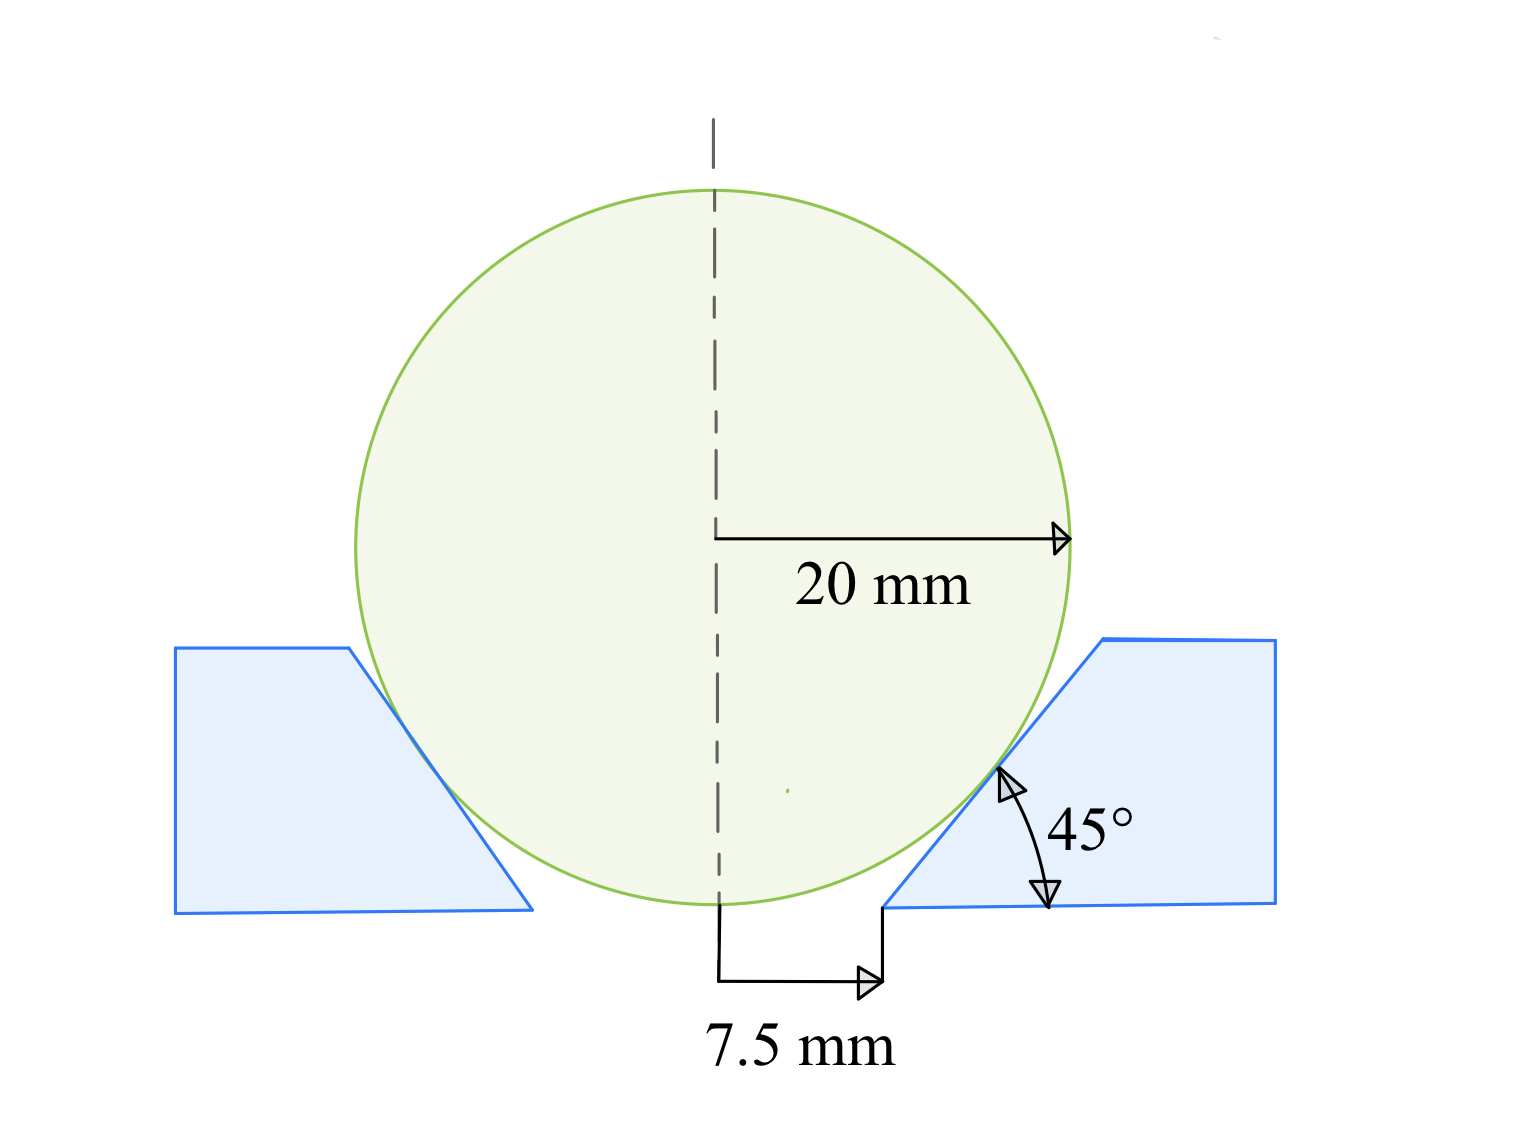
\includegraphics[width=0.5\textwidth]{figures/BallSeatValve/ballseatvalve.jpg}
    \caption{Sketch of ball seat valve.}
    \label{fig:ballseatvalve}
\end{figure}

%%%%%%%%%%%%%%%%%%%%%%%%%%%%%%%%%%%%%%%%%%%%%%%%%%%%%%%%%%%%%%%%%%%%%%%%%%%%%%
                      %%Sealing and leakage%%
%%%%%%%%%%%%%%%%%%%%%%%%%%%%%%%%%%%%%%%%%%%%%%%%%%%%%%%%%%%%%%%%%%%%%%%%%%%%%%%
\section{Sealing and Leakage}
\label{Sealing and Leakage}
The sealing performance of a valve is the ability of the valve's sealing component to prevent the leakage 
of medium. In order to control the flow of the fluids through a pipeline, valves must be installed, and 
the pipeline must be sealed to prevent leakage of the fluids it conveys. In the industrial manufacturing 
process, leaks from valves can have a detrimental influence on economic costs, safety, and environment, 
and can lead to significant production accidents; therefore, valves must have reliable sealing performance 
and meet the operating conditions' requirements 
for leakage. Therefore, it is necessary to investigate the sealing performance and leakage of valves.\\

In theory, the sealing principle of a ball seat valve is that the ball and the seat, both having 
perfectly smooth surfaces, are pressed against each other under load, and the two contact surfaces are 
entirely bonded together to prevent the passage of fluid from the valve in the pipeline, thereby achieving
a seal. In fact, however, it is not possible to obtain a theoretically smooth surface with 
modern machining technology.\cite{Sealing1} Consequently, it is common knowledge that there is no perfectly sealed valve in the world 
and that fluid leakage is bound to occur when the ball and seat are not fully bonded.\\

The sealing of a ball seat valve is determined by a large range of different factors.\cite{fischer2021influence}
For example, it is influenced by the roughness of the contact surfaces. Metallic surfaces are rough 
on a microscopic level.It must have uneven grooves and convex peaks. Due to the surface roughness, two rough 
planes which are apparently at full contact have a reduced real contact area if they 
are investigated using a higher resolution.\cite{fischer2021geometry} This means that when two 
rough sealing surfaces come into contact with each other,
 their highest peaks meet and microscopic channels are formed between the valleys, resulting in a leak.\\

 The sealing is also influenced by the applied forces and pressures on the system. When the load is increased,
  the two convex peaks in contact will be elastoplastically deformed to effectively increase the real contact area, 
  thereby reducing the size of the microscopic channel. However, the space between 
 the two corresponding valleys cannot be entirely eliminated, therefore a perfect seal is not achieved.\cite{Sealing2}
 In addition, the sealing is also influenced by temperature, the viscosity of the fluid in the pipe, etc. 
 In summary, the most important influencing factors that affect leakage can be divided into two main 
 categories: mechanical and hydraulic. Mechanical factors include those that act directly on the sealing 
 position through the valve. In contrast, hydraulic factors are introduced into 
 the system by the fluid. The Table \Ref{tab:influencing factors to valve} provides an overview of the most 
 important influential factors. \cite{PhD-M.S}


    \begin{table}[h!]
        \centering
        \begin{tabular}{||c| c |c |c||} 
         \hline
         Mechanical influencing factor & Hydraulic influencing factors  \\ [0.5ex] 
         \hline\hline
         Contact pressure  & Pressure difference  \\ 
         Macroscopic contact geometry & Temperature  \\
         Microscopic contact geometry & Viscosity \\
         Material hardness & Pollution \\
         Various material influences & Additive influences \\
         Geometric tolerance & Pressure pulsations\\[1ex] 
         \hline
        \end{tabular}
        \caption{The most important influencing factors to valve leakage.\cite{PhD-M.S}}
        \label{tab:influencing factors to valve}
        \end{table}

        It is impractical to discuss all the influencing factors simultaneously to analyze 
        the leakage of the ball seat valve. By controlling variables, the purpose of this study
         is to investigate the effect of the type and the 
        concentration of particles contained in the fluid on the leakage of the ball seat valve.
\chapter{Experiment}
\label{ch:Experiment}
As has already been shown, the sealing of valves is essential for the reliability of 
pipeline transport in hydraulic and pneumatic systems. Leakage can impact the efficiency
 of industrial production and contribute to the occurrence of potential dangers. 
Due to these factors, it is crucial to investigate leaks in metal valves.\\

\section{Test Rig}
\label{Test Rig}
Figure \Ref{fig:TestRig1} depicts a developed experimental platform that was available before this study 
was carried out. A ball seat valve, a water tank, pipelines, an air motor, a hydraulic pump,
and ball valves are its primary components. The medium passing through the pipeline 
consists of distilled water and various types of microscopic particles. Distilled water
was chosen for two primary reasons. First, it comprises a negligible amount of particles,
which has the least potential impact on the particles being analyzed and reduces the 
errors caused in the test results. Also, water has a smaller viscosity as compared to
hydraulic oil, which is usually used in industrial applications. 
The smaller viscosity leads to a higher leakage, which is easier to measure. \cite{fischer2021influence}\\

\begin{figure}[htbp]
    \centering
    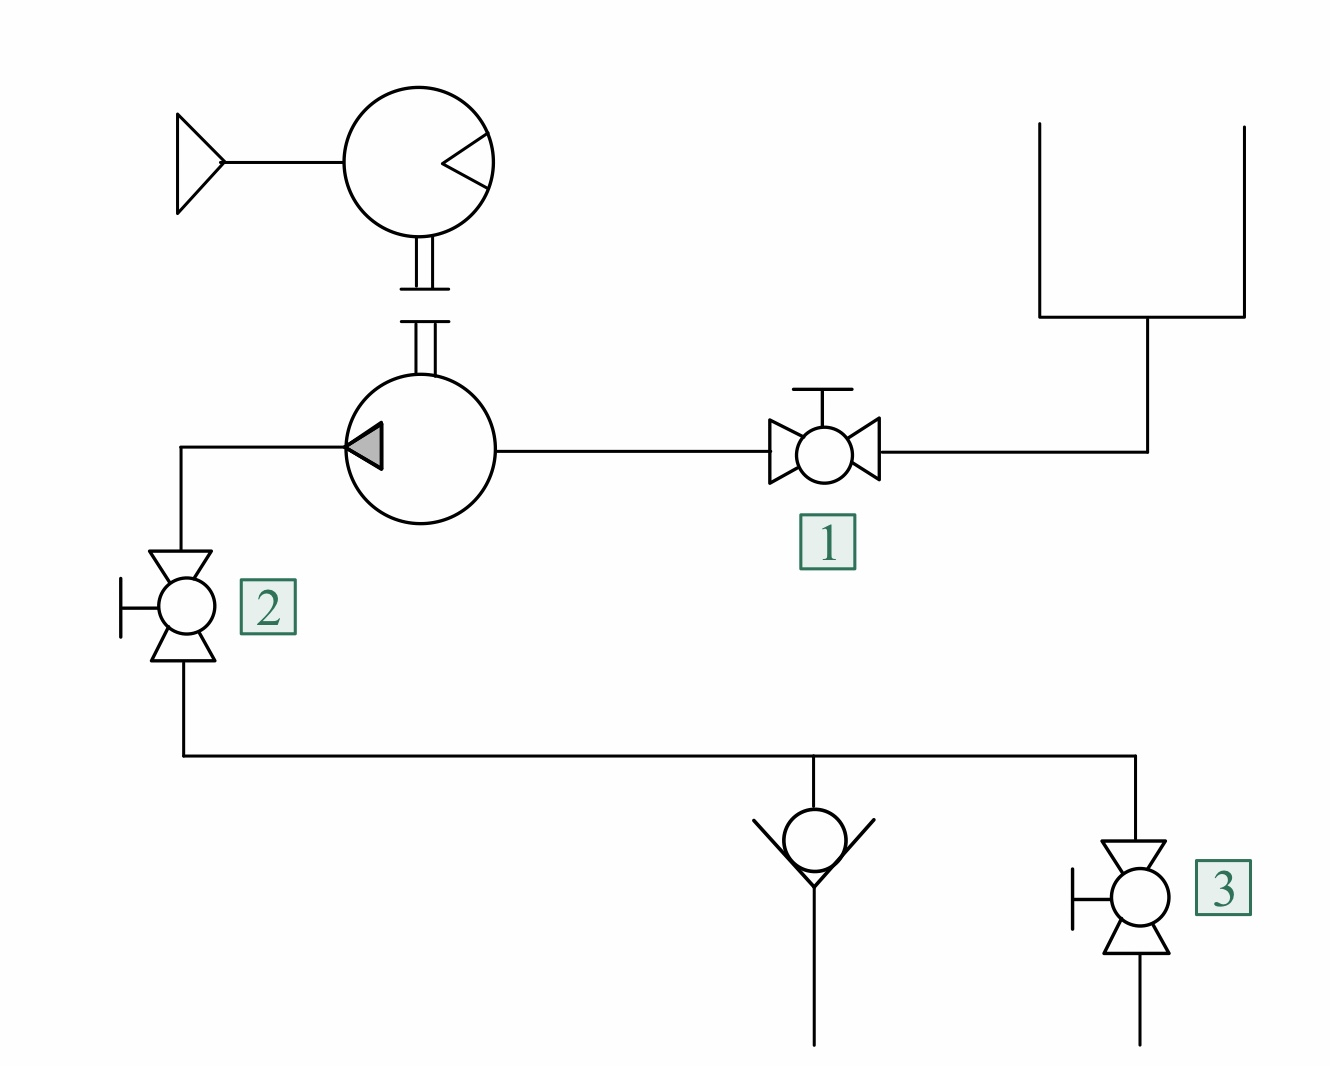
\includegraphics[width=0.5\textwidth]{figures/TestRig/TestRig1.jpg}
    \caption{Sketch of a original available test rig.}
    \label{fig:TestRig1}
\end{figure}

Distilled water and particles will be mixed in a specific proportion. 
Through the water tank, the mixture is pumped into the pipeline, where 
it is transformed into a hydraulic medium and delivered on to the valve. 
Due to the imperfect sealing of the ball seat valve, distilled water can leak 
from a high-pressure environment to a low-pressure environment, i.e., to the 
atmosphere where the relative pressure is zero. This facilitates the detection of leaks, 
and the sealing of the ball seat valve can be analyzed by measuring the amount of leakage.\\

The initial testing platform will be upgraded in order to keep the distilled water and microscopic
 particles in the pipeline as uniformly mixed as feasible. As illustrated in Figure \Ref{fig:TestRig1}, 
 the medium 
 entering the pipe from the tank either leaks into the atmosphere through the valve or flows out as 
 wastewater at the end of the experiment through the opened drain ball valve No. 3 at the pipe's end, 
 indicating that the pipe is not a closed circuit. During the process of measuring the leakage of the 
 ball seat valve, the No. 3 drain valve always remains closed. When the sealing of the ball seat valve 
 is not particularly poor, the amount of leaking fluid will be small, resulting in the mixture entering 
 the pipe only being dynamic when it is just flowing into the pipe. As the mixture fills the pipe, its 
 state gradually becomes static, which is likely to cause tiny particles to settle downwards due to their
  own weight, thus accumulating in the pipe and failing to mix evenly with the distilled water, resulting 
  in the actual concentration of particles in the mixture passing through the ball seat valve 
 deviating too greatly from the initial set concentration added to the water tank.\\

 The test rig was improved by connecting the end of the original pipe to the tank with a new section of
  pipe and a ball valve No. 4, as illustrated in Figure \Ref{fig:TestRig2}. With the ball valve No. 4 partially open, 
  the entire pipe forms a closed circuit, and the mixture is able to circulate through the pipe under 
  the action of the hydraulic pump. The microscopic particles also gain more kinetic energy, decreasing 
  the probability of deposition in the pipe and thus increasing the degree of mixing with distilled water. 
  Special consideration should also be given to the fact that the ball valve No. 4 should only be partially 
  opened and not entirely opened; otherwise, it will be challenging for the hydraulic system 
  to attain and maintain the desired pressure level.

  \begin{figure}[htbp]
    \centering
    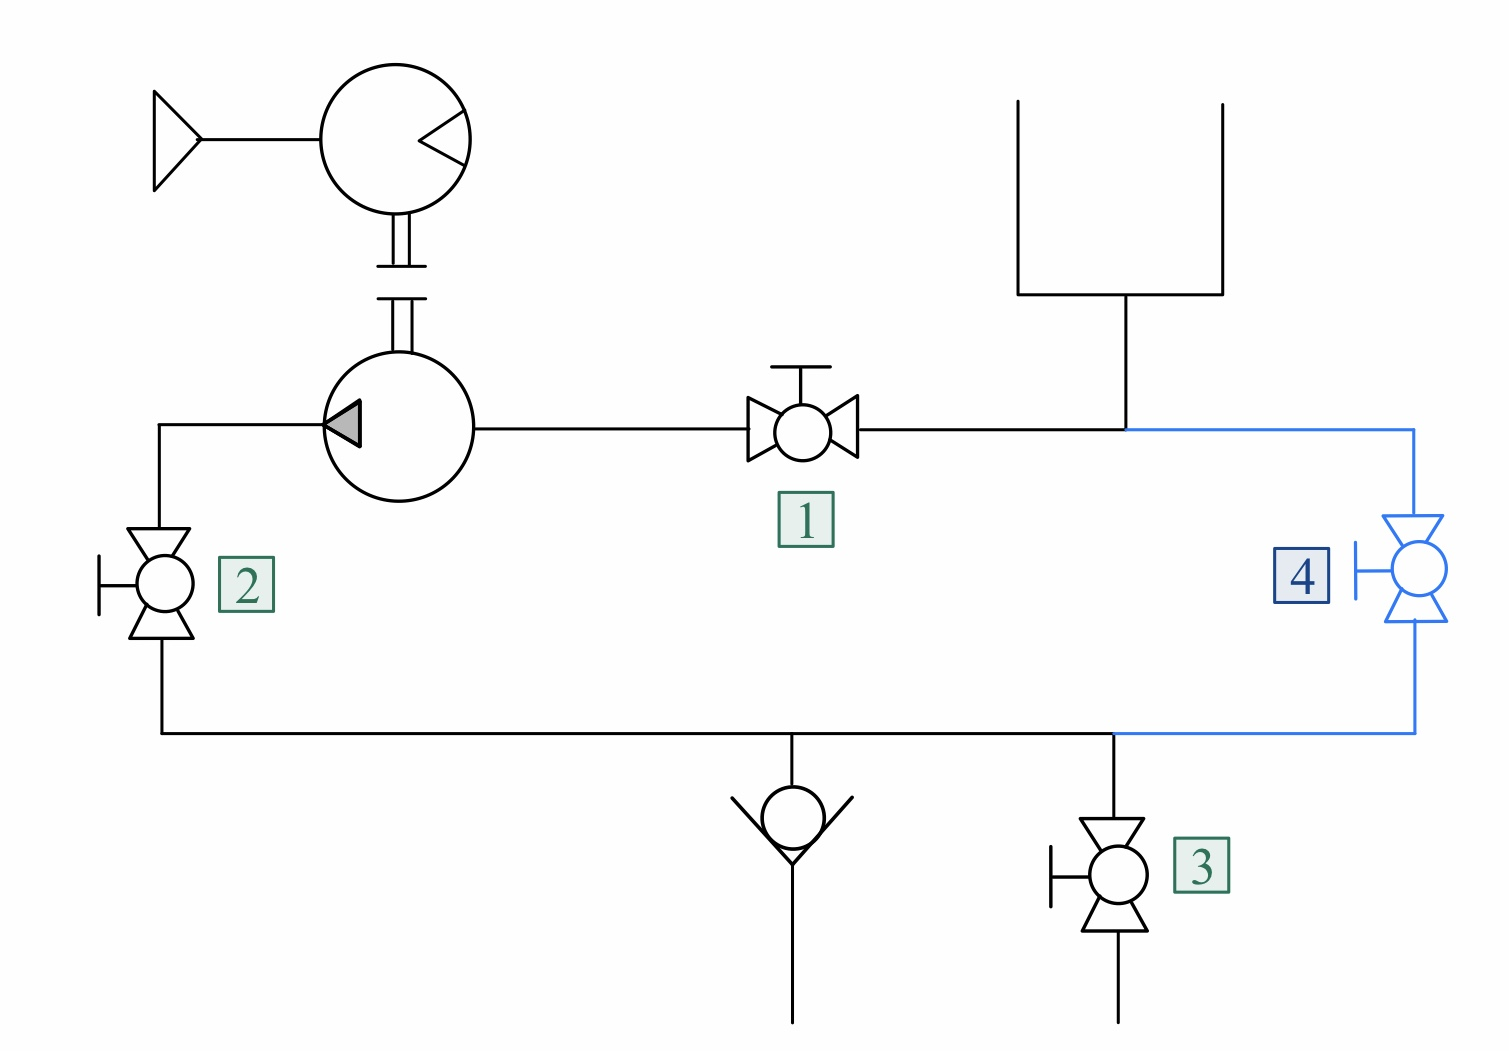
\includegraphics[width=0.5\textwidth]{figures/TestRig/TestRig2.jpg}
    \caption{Sketch of a improved test rig.}
    \label{fig:TestRig2}
\end{figure}
\newpage
\chapter{Result and Discussionn}
\label{Result and discussion}



\begin{appendix}

\listoffigures
\listoftables
\listoflistings

\bibliographystyle{IEEEtran}
\bibliography{IEEEabrv,bib/IEEEtranBST,bib/your.bib}


\end{appendix}

\end{document}


%%%%%%%%%%%%%%%%%%%%%%%%%%%%%%%%%%%%%%%%%%%%%%%%%%%%%%%%%%%%%%%%%%%%%%%%%%%%%%%
%                          END OF THE DOCUMENT                                %
%%%%%%%%%%%%%%%%%%%%%%%%%%%%%%%%%%%%%%%%%%%%%%%%%%%%%%%%%%%%%%%%%%%%%%%%%%%%%%%
